\documentclass{article}

\usepackage{fullpage}
\usepackage{url}
\usepackage{bbm}
\usepackage{graphicx}
\usepackage{amsmath}
\usepackage{physics}
\usepackage{mathtools}
\usepackage{bbold}
\usepackage{slashed}
\usepackage{pxfonts}
\usepackage{multicol}
\usepackage{mathptmx}
\usepackage{simplewick}
\usepackage{placeins}
\usepackage{booktabs}
\usepackage{tikz}
\usepackage[compat=1.1.0]{tikz-feynman}

\usepackage{lmodern}
\usepackage[T1]{fontenc}
\usepackage[fontsize=13.5pt]{fontsize}

\DeclareMathOperator{\erfi}{erfi}
\newcommand{\R}{\ensuremath{\mathbb{R}}}
\newcommand{\C}{\ensuremath{\mathbb{C}}}


\title{QFT1 Formulas}
\author{Idan Stark}

\begin{document}
\maketitle

\section{A theory of two scalars in $5+1$ dimensions}
\subsection{Counter terms}
We take the most general form of the Lagrangian with all renormlizable operators, i.e. all operators with dimension $\Delta \le 3$. There are no symmetries, so this includes:
\begin{equation}
\begin{gathered}
    \mathcal{L} = \mathcal{L}_0 + \sum_i^2 \left(\frac{1}{2}\delta_{z_i}\left(\partial_\mu \phi_i\right)^2 - \frac{1}{2}\delta_{m_i}\phi_i^2\right) - \\ - \delta_0\phi_1\phi_2 - \frac{1}{2}\delta_1\phi_1^2\phi_2 - \frac{1}{2}\delta_2\phi_1\phi_2^2 - \frac{1}{6}\delta_3\phi_2^3 - \frac{1}{6}\delta_4\phi_1^3
\end{gathered}
\end{equation}
\subsection{The correlation function $\langle \phi(x) \rangle$}
The correlation function $\langle \phi(x) \rangle$, in one loop order, requires an odd number of $\phi_1$ fields in the term, to contract with it. The only such term in the original Lagrangian is $\frac{\lambda_2}{2}\phi_1\phi_2^2$. This is a tadpole diagram, with only one contraction option, giving:
\begin{equation}
    \langle \tilde{\phi}(p) \rangle = \frac{-i\lambda_2 \delta^{(6)}(p)}{2} \frac{i}{p^2 - m_1^2 + i\epsilon} \int \frac{d^6k}{(2\pi)^6}\frac{i}{k^2 - m_2^2 + i\epsilon}
\end{equation}
This diverges quartically as $\frac{d^6k}{k^2} \sim k^4$, so we will use dimensional regularization:
\begin{equation}
    \int \frac{d^6k}{(2\pi)^6}\frac{i}{k^2 - m_2^2 + i\epsilon} \rightarrow \int \frac{d^dk}{(2\pi)^d}\frac{i}{k^2 - m_2^2 + i\epsilon}
\end{equation}
Moving to Euclidean space:
\begin{equation}
    \int \frac{d^dk}{(2\pi)^d}\frac{i}{k^2 - m_2^2 + i\epsilon} = \int \frac{d^dk_E}{(2\pi)^d}\frac{1}{p_E^2 + m_2^2 + i\epsilon}
\end{equation}
And using the known integral for $\Delta = m_2^2, n = 1$:
\begin{equation}
    \langle \tilde{\phi}(p) \rangle = \frac{\lambda_2\delta^{(d)}(p)}{2(4\pi)^d/2}\frac{1}{p^2 - m_1^2 + i\epsilon}\frac{\Gamma(1 - \frac{d}{2})}{\Gamma(1)}\Delta^{\frac{d}{2}-1}
\end{equation}
\begin{equation}
    \langle \tilde{\phi}(p) \rangle = \frac{1}{p^2 - m_1^2 + i\epsilon}\frac{\Gamma(1 - \frac{d}{2})}{2(4\pi)^d/2} \frac{1}{\Gamma(1)}m_2^{d - 2}\lambda_2\delta^{(d)}(p)
\end{equation}
Since
\begin{equation}
    \left[\frac{1}{p^2 - m_1^2 + i\epsilon}\right] = -2
    \qquad
    \left[m_2\right] = 1
    \qquad
    \left[\lambda_2\right] = 3 - \frac{d}{2}
    \qquad
    \left[\delta^{(d)}(p)\right] = -d
\end{equation}
The dimension of the correlation function is:
\begin{equation}
    \left[\langle \tilde{\phi}(p) \rangle\right] = -2 + (d-2)\left[m_2\right] + \left[\lambda_2\right] - d = -\frac{d + 2}{2}
\end{equation}
Which, after performing the Fourier transform back to $\phi(x)$, gives (with the measure of the fourier integral having mass dimension $d$), exactly the field mass dimension $\frac{d - 2}{2}$.
\newline
As we can see, this result is linear in $\lambda_2$, so a counter term of the same form $\phi_1\phi_2^2$ will give similar result. Setting $\delta_2 = -\lambda_2$ will give the opposite contribution, making the correlation function vanish.
\subsection{The 1PI propagators}
\subsubsection{$\langle \phi_1(p)\phi_1(-p) \rangle$}
In this case there are two contributing diagrams:
\begin{center}
\begin{tikzpicture}[baseline=(current bounding box.center)]
  \begin{feynman}
    \vertex[dot] (v1) at (-0.5,0) {};
    \vertex[dot] (v2) at (0.5,0) {};
    \vertex (i1) at (-1.5,0);
    \vertex (f1) at (1.5,0);
    \draw[plain] (i1) -- (v1);
    \draw[plain] (v2) -- (f1);
    \draw[scalar] (v1) to[out=90, in=90] (v2);
    \draw[scalar] (v2) to[out=-90, in=-90] (v1);
  \end{feynman}
\end{tikzpicture}
\hspace{0.5cm}
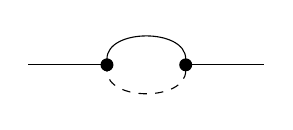
\begin{tikzpicture}[baseline=(current bounding box.center)]
  \begin{feynman}
    \vertex[dot] (v1) at (-0.5,0) {};
    \vertex[dot] (v2) at (0.5,0) {};
    \vertex (i1) at (-1.5,0);
    \vertex (f1) at (1.5,0);
    \draw[plain] (i1) -- (v1);
    \draw[plain] (v2) -- (f1);
    \draw[plain] (v1) to[out=90, in=90] (v2);
    \draw[scalar] (v2) to[out=-90, in=-90] (v1);
  \end{feynman}
\end{tikzpicture}
\end{center}
They give:
\begin{equation}
\begin{gathered}
    -i\Sigma_{11}(p) = \frac{(-i\lambda_2)^2}{2}\int\frac{d^6k}{(2\pi)^k}\frac{i}{k^2 - m_2^2 + i\epsilon}\frac{i}{(p - k)^2 - m_2^2 + i\epsilon} + \\ +
    \frac{(-i\lambda_1)^2}{2}\int\frac{d^6k}{(2\pi)^k}\frac{i}{k^2 - m_1^2 + i\epsilon}\frac{i}{(p - k)^2 - m_2^2 + i\epsilon}
\end{gathered}
\end{equation}
Moving to $d$ dimensions and using the given integral:
\begin{equation}
    -i\Sigma_{11}(p) = i \frac{\Gamma\left(2 - \frac{d}{2}\right)}{2(2\pi)^{d/2}}\int_0^1dx \left[\frac{\lambda_2^2}{\left(m_2^2 - x(1 - x)p^2\right)^{2 - \frac{d}{2}}} + \frac{\lambda_1^2}{\left(xm_1^2 + (1 - x)m_2^2 - x(1 - x)p^2\right)^{2 - \frac{d}{2}}}\right]
\end{equation} 
\subsubsection{$\langle \phi_1(p)\phi_2(-p) \rangle$}
This case is very similar, with again two diagrams:
\begin{center}
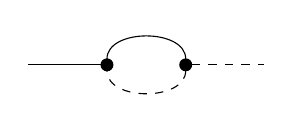
\begin{tikzpicture}[baseline=(current bounding box.center)]
  \begin{feynman}
    \vertex[dot] (v1) at (-0.5,0) {};
    \vertex[dot] (v2) at (0.5,0) {};
    \vertex (i1) at (-1.5,0);
    \vertex (f1) at (1.5,0);
    \draw[plain] (i1) -- (v1);
    \draw[scalar] (v2) -- (f1);
    \draw[plain] (v1) to[out=90, in=90] (v2);
    \draw[scalar] (v2) to[out=-90, in=-90] (v1);
  \end{feynman}
\end{tikzpicture}
\hspace{0.5cm}
\begin{tikzpicture}[baseline=(current bounding box.center)]
  \begin{feynman}
    \vertex[dot] (v1) at (-0.5,0) {};
    \vertex[dot] (v2) at (0.5,0) {};
    \vertex (i1) at (-1.5,0);
    \vertex (f1) at (1.5,0);
    \draw[plain] (i1) -- (v1);
    \draw[scalar] (v2) -- (f1);
    \draw[scalar] (v1) to[out=90, in=90] (v2);
    \draw[scalar] (v2) to[out=-90, in=-90] (v1);
  \end{feynman}
\end{tikzpicture}
\end{center}
This is identical to the first case, only with different coefficients matching the vertices, and we need to make sure the internal propagators have the correct mass:
\begin{equation}
    -i\Sigma_{12}(p) = i \frac{\Gamma\left(2 - \frac{d}{2}\right)}{2(2\pi)^{d/2}}\int_0^1dx \left[\frac{\lambda_2\lambda_3}{\left(m_2^2 - x(1 - x)p^2\right)^{2 - \frac{d}{2}}} + \frac{\lambda_1\lambda_2}{\left(xm_1^2 + (1 - x)m_2^2 - x(1 - x)p^2\right)^{2 - \frac{d}{2}}}\right]
\end{equation}
\subsection{Imaginary part of $\Sigma_{11}$}
In order to have an imaginary part, there should be physical intermidiate states. In the correlation function $\langle \phi_1(p)\phi_1(-p) \rangle$, this means there are is enough momentum to create either two $\phi_2$ particles, or a $\phi_1$ and a $\phi_2$ particle:
\begin{equation}
    p^2 \ge \min(4m_2^2, (m_1 + m_2)^2) = \begin{cases}
        4m_2^2 & m_1 < m_2 \\ (m_1 + m_2)^2 & m_2 < m_1
    \end{cases}
\end{equation}
\subsection{Counter terms}
The 2 point correlation function gets contribution from the kinetic and mass counter terms:
\begin{equation}
\begin{gathered}
    \Sigma_{11}(p) = \frac{\Gamma\left(2 - \frac{d}{2}\right)}{2(2\pi)^{d/2}}\int_0^1dx \left[\frac{\lambda_2^2}{\left(m_2^2 - x(1 - x)p^2\right)^{2 - \frac{d}{2}}} + \frac{\lambda_1^2}{\left(xm_1^2 + (1 - x)m_2^2 - x(1 - x)p^2\right)^{2 - \frac{d}{2}}}\right] + \\ +
    \delta_{z_1}p^2 - \delta_{m_1}
\end{gathered}
\end{equation}
Deriving by $p^2$ gives:
\begin{equation}
\begin{gathered}
    \frac{\partial}{\partial p^2} \Sigma_{11}(p) = \delta_{z_1} + \\ +
    \left(2 - \frac{d}{2}\right)\frac{\Gamma\left(2 - \frac{d}{2}\right)}{2(2\pi)^{d/2}}\int_0^1dx \left[\frac{\lambda_2^2x(1 - x)}{\left(m_2^2 - x(1 - x)p^2\right)^{3 - \frac{d}{2}}} + \frac{\lambda_1^2x(1 - x)}{\left(xm_1^2 + (1 - x)m_2^2 - x(1 - x)p^2\right)^{3 - \frac{d}{2}}}\right]
\end{gathered}
\end{equation}
Requiring the derivative to be zero for $p^2 = M^2$ gives:
\begin{equation}
    \delta_{z_1} = \left(\frac{d}{2} - 2\right)\frac{\Gamma\left(2 - \frac{d}{2}\right)}{2(2\pi)^{d/2}}\int_0^1dx \left[\frac{\lambda_2^2x(1 - x)}{\left(m_2^2 - x(1 - x)M^2\right)^{3 - \frac{d}{2}}} + \frac{\lambda_1^2x(1 - x)}{\left(xm_1^2 + (1 - x)m_2^2 - x(1 - x)M^2\right)^{3 - \frac{d}{2}}}\right]
\end{equation}
Similarly from the $\Sigma_{12}$ 1PI, we get:
\begin{equation}
    \delta_{z_2} = \left(\frac{d}{2} - 2\right)\frac{\Gamma\left(2 - \frac{d}{2}\right)}{2(2\pi)^{d/2}}\int_0^1dx \left[\frac{\lambda_2\lambda_3x(1 - x)}{\left(m_2^2 - x(1 - x)M^2\right)^{3 - \frac{d}{2}}} + \frac{\lambda_1\lambda_2x(1 - x)}{\left(xm_1^2 + (1 - x)m_2^2 - x(1 - x)M^2\right)^{3 - \frac{d}{2}}}\right]
\end{equation}
\subsection{The physical masses of the particles}
\subsubsection{Stability of the particles}
A prticle in this theory is unstable only if it can decay into a pair of the other particle. Therefore, for $\tilde{m} < 2m$ and $m < 2\tilde{m}$, the particles are stable. This gives:
\begin{equation}
    \frac{1}{2} < \frac{m}{\tilde{m}} < 2
\end{equation}
\subsubsection{The poles and imaginary part of $\langle \phi_1\phi_1 \rangle$}
Since the particles are a generic mix of the two fields, inverting the transformation means that each field is a generic combination of the two particle fields. In other words, the propagator of each field will have poles for both physical masses $m, \tilde{m}$.
\newline
Additionally, the $\langle \phi_1\phi_1 \rangle$ propagator will have an imaginary part if it has a physical intermidiate state, which means that it will create two physical particles. We take the one with the smaller mass:
\begin{equation}
    p^2 \ge 4\min(m, \tilde{m})^2 = \begin{cases}
         4m^2 & m < \tilde{m} \\ 4\tilde{m}^2 & \tilde{m} < m
    \end{cases}
\end{equation}
\subsection{The beta functions of $\lambda_1$, $\lambda_2$, and $\lambda_3$}
We saw in the tutorial that for the $\phi^3$ theory there is a single diagram contributing to the vertex correction in order $\lambda^3$, which gave us, for scales much larger then the masses:
\begin{equation}
    -\frac{\lambda^3}{(4\pi)^3}
\end{equation}
In the $\langle \phi_2 \phi_2 \phi_2 \rangle$ case of this theory, we have eight different diagrams:
\begin{center}
\begin{tikzpicture}[baseline=(current bounding box.center)]
  \begin{feynman}
    \vertex (v1) at (-0.5, 1);
    \vertex (v2) at (-0.5, -1);
    \vertex (v3) at (1, 0);
    \vertex (i1) at (-1, 2);
    \vertex (i2) at (-1, -2);
    \vertex (f2) at (2, 0);
    \draw[scalar] (v1) -- (v2);
    \draw[scalar] (i2) -- (v2);
    \draw[scalar] (v2) -- (v3);
    \draw[scalar] (v3) -- (v1);
    \draw[scalar] (v1) -- (i1);
    \draw[scalar] (v3) -- (f2);
  \end{feynman}
\end{tikzpicture}
\hspace{1cm}
\begin{tikzpicture}[baseline=(current bounding box.center)]
  \begin{feynman}
    \vertex (v1) at (-0.5, 1);
    \vertex (v2) at (-0.5, -1);
    \vertex (v3) at (1, 0);
    \vertex (i1) at (-1, 2);
    \vertex (i2) at (-1, -2);
    \vertex (f2) at (2, 0);
    \draw[scalar] (v1) -- (v2);
    \draw[scalar] (i2) -- (v2);
    \draw[plain] (v2) -- (v3);
    \draw[scalar] (v3) -- (v1);
    \draw[scalar] (v1) -- (i1);
    \draw[scalar] (v3) -- (f2);
  \end{feynman}
\end{tikzpicture}
\hspace{1cm}
\begin{tikzpicture}[baseline=(current bounding box.center)]
  \begin{feynman}
    \vertex (v1) at (-0.5, 1);
    \vertex (v2) at (-0.5, -1);
    \vertex (v3) at (1, 0);
    \vertex (i1) at (-1, 2);
    \vertex (i2) at (-1, -2);
    \vertex (f2) at (2, 0);
    \draw[scalar] (v1) -- (v2);
    \draw[scalar] (i2) -- (v2);
    \draw[plain] (v2) -- (v3);
    \draw[plain] (v3) -- (v1);
    \draw[scalar] (v1) -- (i1);
    \draw[scalar] (v3) -- (f2);
  \end{feynman}
\end{tikzpicture}
\hspace{1cm}
\begin{tikzpicture}[baseline=(current bounding box.center)]
  \begin{feynman}
    \vertex (v1) at (-0.5, 1);
    \vertex (v2) at (-0.5, -1);
    \vertex (v3) at (1, 0);
    \vertex (i1) at (-1, 2);
    \vertex (i2) at (-1, -2);
    \vertex (f2) at (2, 0);
    \draw[plain] (v1) -- (v2);
    \draw[scalar] (i2) -- (v2);
    \draw[plain] (v2) -- (v3);
    \draw[plain] (v3) -- (v1);
    \draw[scalar] (v1) -- (i1);
    \draw[scalar] (v3) -- (f2);
  \end{feynman}
\end{tikzpicture}
\end{center}
Where the center two diagrams have each three different positions for the internal $\phi_1$ propagator. From left to right, they give the contributions:
\begin{equation}
    \beta(\lambda_3) = -2\cdot\frac{1}{2}\frac{\lambda_3^3}{(2\pi)^3}
    -2\cdot3\cdot \frac{1}{9} \frac{\lambda_2^2\lambda_3}{(2\pi)^3}
    -2\cdot3\cdot\frac{2}{27}\frac{\lambda_1\lambda_2^2}{(2\pi)^3}
    -2\cdot\frac{1}{27}\frac{\lambda_1^3}{(2\pi)^3}
\end{equation}
\begin{equation}
    \beta(\lambda_3) = -\frac{1}{(2\pi)^3} \left[
        \lambda_3^3 + \frac{2}{3}\lambda_2^2\lambda_3 +
        \frac{4}{9}\lambda_1\lambda_2^2 + \frac{2}{27}\lambda_1^3
    \right]
\end{equation}
Similarly, each of the other vertices has four diagrams contributing to its correction. For the $\langle \phi_1 \phi_1 \phi_2 \rangle$ correlation function, the diagrams are:
\begin{center}
\begin{tikzpicture}[baseline=(current bounding box.center)]
  \begin{feynman}
    \vertex (v1) at (-0.5, 1);
    \vertex (v2) at (-0.5, -1);
    \vertex (v3) at (1, 0);
    \vertex (i1) at (-1, 2);
    \vertex (i2) at (-1, -2);
    \vertex (f2) at (2, 0);
    \draw[plain] (v1) -- (v2);
    \draw[plain] (i2) -- (v2);
    \draw[scalar] (v2) -- (v3);
    \draw[scalar] (v3) -- (v1);
    \draw[plain] (v1) -- (i1);
    \draw[scalar] (v3) -- (f2);
  \end{feynman}
\end{tikzpicture}
\hspace{1cm}
\begin{tikzpicture}[baseline=(current bounding box.center)]
  \begin{feynman}
    \vertex (v1) at (-0.5, 1);
    \vertex (v2) at (-0.5, -1);
    \vertex (v3) at (1, 0);
    \vertex (i1) at (-1, 2);
    \vertex (i2) at (-1, -2);
    \vertex (f2) at (2, 0);
    \draw[scalar] (v1) -- (v2);
    \draw[plain] (i2) -- (v2);
    \draw[scalar] (v2) -- (v3);
    \draw[plain] (v3) -- (v1);
    \draw[plain] (v1) -- (i1);
    \draw[scalar] (v3) -- (f2);
  \end{feynman}
\end{tikzpicture}
\hspace{1cm}
\begin{tikzpicture}[baseline=(current bounding box.center)]
  \begin{feynman}
    \vertex (v1) at (-0.5, 1);
    \vertex (v2) at (-0.5, -1);
    \vertex (v3) at (1, 0);
    \vertex (i1) at (-1, 2);
    \vertex (i2) at (-1, -2);
    \vertex (f2) at (2, 0);
    \draw[scalar] (v1) -- (v2);
    \draw[plain] (i2) -- (v2);
    \draw[scalar] (v2) -- (v3);
    \draw[scalar] (v3) -- (v1);
    \draw[plain] (v1) -- (i1);
    \draw[scalar] (v3) -- (f2);
  \end{feynman}
\end{tikzpicture}
\hspace{1cm}
\begin{tikzpicture}[baseline=(current bounding box.center)]
  \begin{feynman}
    \vertex (v1) at (-0.5, 1);
    \vertex (v2) at (-0.5, -1);
    \vertex (v3) at (1, 0);
    \vertex (i1) at (-1, 2);
    \vertex (i2) at (-1, -2);
    \vertex (f2) at (2, 0);
    \draw[scalar] (v1) -- (v2);
    \draw[plain] (i2) -- (v2);
    \draw[plain] (v2) -- (v3);
    \draw[plain] (v3) -- (v1);
    \draw[plain] (v1) -- (i1);
    \draw[scalar] (v3) -- (f2);
  \end{feynman}
\end{tikzpicture}
\end{center}
Where the second diagram has two permutations of the internal propagators. This gives the beta function:
\begin{equation}
    \beta(\lambda_1) = -\frac{1}{(2\pi)^3}\left[\frac{8}{9}\lambda_1^2\lambda_3 + \frac{8}{27}\lambda_1\lambda_2^2 + 
    \frac{4}{27}\lambda_1^3 + \frac{2}{9}\lambda_2^2\lambda_3^2\right]
\end{equation}
And for $\langle \phi_2 \phi_2 \phi_1 \rangle$, the diagrams are:
\begin{center}
\begin{tikzpicture}[baseline=(current bounding box.center)]
  \begin{feynman}
    \vertex (v1) at (-0.5, 1);
    \vertex (v2) at (-0.5, -1);
    \vertex (v3) at (1, 0);
    \vertex (i1) at (-1, 2);
    \vertex (i2) at (-1, -2);
    \vertex (f2) at (2, 0);
    \draw[scalar] (v1) -- (v2);
    \draw[scalar] (i2) -- (v2);
    \draw[scalar] (v2) -- (v3);
    \draw[scalar] (v3) -- (v1);
    \draw[scalar] (v1) -- (i1);
    \draw[plain] (v3) -- (f2);
  \end{feynman}
\end{tikzpicture}
\hspace{1cm}
\begin{tikzpicture}[baseline=(current bounding box.center)]
  \begin{feynman}
    \vertex (v1) at (-0.5, 1);
    \vertex (v2) at (-0.5, -1);
    \vertex (v3) at (1, 0);
    \vertex (i1) at (-1, 2);
    \vertex (i2) at (-1, -2);
    \vertex (f2) at (2, 0);
    \draw[plain] (v1) -- (v2);
    \draw[scalar] (i2) -- (v2);
    \draw[scalar] (v2) -- (v3);
    \draw[scalar] (v3) -- (v1);
    \draw[scalar] (v1) -- (i1);
    \draw[plain] (v3) -- (f2);
  \end{feynman}
\end{tikzpicture}
\hspace{1cm}
\begin{tikzpicture}[baseline=(current bounding box.center)]
  \begin{feynman}
    \vertex (v1) at (-0.5, 1);
    \vertex (v2) at (-0.5, -1);
    \vertex (v3) at (1, 0);
    \vertex (i1) at (-1, 2);
    \vertex (i2) at (-1, -2);
    \vertex (f2) at (2, 0);
    \draw[scalar] (v1) -- (v2);
    \draw[scalar] (i2) -- (v2);
    \draw[scalar] (v2) -- (v3);
    \draw[plain] (v3) -- (v1);
    \draw[scalar] (v1) -- (i1);
    \draw[plain] (v3) -- (f2);
  \end{feynman}
\end{tikzpicture}
\hspace{1cm}
\begin{tikzpicture}[baseline=(current bounding box.center)]
  \begin{feynman}
    \vertex (v1) at (-0.5, 1);
    \vertex (v2) at (-0.5, -1);
    \vertex (v3) at (1, 0);
    \vertex (i1) at (-1, 2);
    \vertex (i2) at (-1, -2);
    \vertex (f2) at (2, 0);
    \draw[plain] (v1) -- (v2);
    \draw[scalar] (i2) -- (v2);
    \draw[scalar] (v2) -- (v3);
    \draw[plain] (v3) -- (v1);
    \draw[scalar] (v1) -- (i1);
    \draw[plain] (v3) -- (f2);
  \end{feynman}
\end{tikzpicture}
\end{center}
Where the thid and fourth diagrams have two permutations of the internal propagators. This gives the beta function:
\begin{equation}
    \beta(\lambda_2) = -\frac{1}{(2\pi)^3}\left[\frac{2}{3}\lambda_2^2\lambda_3 + \frac{4}{27}\lambda_2^3 + 
    \frac{2}{9}\lambda_1\lambda_2\lambda_3 + \frac{4}{27}\lambda_1^2\lambda_2\right]
\end{equation}
\subsection{Linear terms in the coupling of in the beta functions}
While in the perturbative sense, all terms are of order $\lambda^3$, there are terms in the beta functions that are linear to each of the $\lambda_i$.
\subsection{The remaining coupling}
The last dimensionless coupling would be the coupling for the $\phi_1^3$ operator, named $\lambda_4$ by our convention. the one loop contribution to the correction has just two diagrams:
\begin{center}
\begin{tikzpicture}[baseline=(current bounding box.center)]
  \begin{feynman}
    \vertex (v1) at (-0.5, 1);
    \vertex (v2) at (-0.5, -1);
    \vertex (v3) at (1, 0);
    \vertex (i1) at (-1, 2);
    \vertex (i2) at (-1, -2);
    \vertex (f2) at (2, 0);
    \draw[scalar] (v1) -- (v2);
    \draw[plain] (i2) -- (v2);
    \draw[scalar] (v2) -- (v3);
    \draw[scalar] (v3) -- (v1);
    \draw[plain] (v1) -- (i1);
    \draw[plain] (v3) -- (f2);
  \end{feynman}
\end{tikzpicture}
\hspace{1cm}
\begin{tikzpicture}[baseline=(current bounding box.center)]
  \begin{feynman}
    \vertex (v1) at (-0.5, 1);
    \vertex (v2) at (-0.5, -1);
    \vertex (v3) at (1, 0);
    \vertex (i1) at (-1, 2);
    \vertex (i2) at (-1, -2);
    \vertex (f2) at (2, 0);
    \draw[plain] (v1) -- (v2);
    \draw[plain] (i2) -- (v2);
    \draw[scalar] (v2) -- (v3);
    \draw[scalar] (v3) -- (v1);
    \draw[plain] (v1) -- (i1);
    \draw[plain] (v3) -- (f2);
  \end{feynman}
\end{tikzpicture}
\end{center}
Where the second diagram again has three permutation of the internal propagators. This gives the beta function:
\begin{equation}
    \beta(\lambda_4) = -\frac{1}{(2\pi)^3}\left[\frac{2}{27}\lambda_2^3 + \frac{4}{9}\lambda_1^2\lambda_2\right]
\end{equation}
\subsection{The $\lambda_2 = 0$ case}
\subsubsection{The symmetry}
This gives the Lagrangian
\begin{equation}
    L = \sum_{i=1}^2 \left(\frac{1}{2}\left(\partial_m \phi_i\right)^2 - \frac{1}{2}m_i^2\phi_i^2\right) - \frac{1}{2}\lambda_1\phi_1^2\phi_2 - \frac{1}{6}\lambda_3\phi_2^3
\end{equation}
This theory has a symmetry:
\begin{equation}
    \phi_1 \rightarrow -\phi_1
\end{equation}
\subsubsection{The consistancy of the results from previous sections}
We can see that if $\lambda_2 = 0$ for some scale $M$, then the beta function for both $\lambda_2$ and $\lambda_4$ is zero, and thus these terms will not be generated by the RG flow, so these results are consistant with the symmetry.
\subsubsection{The change is reulsts to f (1.6)}
Since the fields do not mix (we saw that in the first term I can copy the results here, but basically $\langle \phi_1 \phi_2 \rangle = -\langle \phi_1 \phi_2 \rangle$ from the path integral with integration variable change), then the masses aer $m_1$ and $m_2$.
\newline
The result of the first section is the same: for a particle to be stable it cannot decay into the other kind of particle through the interactions, meaning that for both to be stable we require:
\begin{equation}
    \frac{1}{2} < \frac{m_1}{m_2} < 2
\end{equation}
For the second part, now the poles of the $\Sigma_{ii}$ 1PI will only be for $m_1$, and it will have an imaginary part by the same condition:
\begin{equation}
    p^2 > 4min(m_1, m_2)^2 = \begin{cases}
        4m_1^2 & m_1 < m_2 \\ 4m_1^2 & m_2 < m_1
    \end{cases}
\end{equation}

\newpage
\section{Photon-photon scattering in scalar QED}
\subsection{The effective photon action}
The most general term that depends on the photon alone that is gauge invariant and Lorentz invariant is $F_{\mu\nu}$. This term is linear i $A_\mu$, and so to adhere to $A_\mu \rightarrow -A_\mu$ symmetry, we must take even powers of it. This means that after the kinetic term, the term with the lowest dimension is the quartic term:
\begin{equation}
    \mathcal{L}_A = -\frac{1}{4}F_{\mu\nu}^2 - \frac{g}{16}F_{\mu\nu}^4
\end{equation}
\subsection{The first order contiburing diagrams}
We work in Feynman gauge, but since it only contributes to the photon propagator, it wouldn't change the value of this result.
\newline
Since there are two types of verties contributing to this process at one-loop order (from the operators $A^2\phi^2$ and $A\phi^2$), there are three families of diagrams: diagrams with all photons interacting with the scalar fields alone, diagrams where all photons interact with the scalar fields in pairs, and diagrams where two photons interact in a pair and two interact alone:
\begin{center}
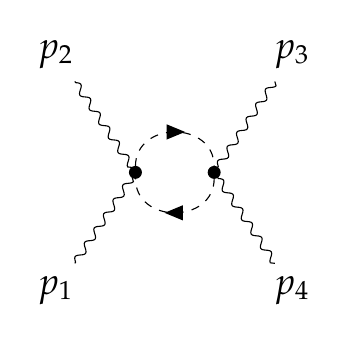
\begin{tikzpicture}[baseline=(current bounding box.center)]
  \begin{feynman}
    \vertex[dot] (v1) at (-0.5,0) {};
    \vertex[dot] (v2) at (0.5,0) {};
    \vertex (i1) at (-1.5, -1.5) {$p_1$};
    \vertex (i2) at (-1.5, 1.5) {$p_2$};
    \vertex (f1) at (1.5, 1.5) {$p_3$};
    \vertex (f2) at (1.5, -1.5) {$p_4$};
    \draw[photon] (i2) -- (v1);
    \draw[photon] (i1) -- (v1);
    \draw[photon] (v2) -- (f1);
    \draw[photon] (v2) -- (f2);
    \draw[charged scalar] (v1) to[out=90, in=90, looseness=1.5] (v2);
    \draw[charged scalar] (v2) to[out=-90, in=-90, looseness=1.5] (v1);
  \end{feynman}
\end{tikzpicture}
\hspace{1cm}
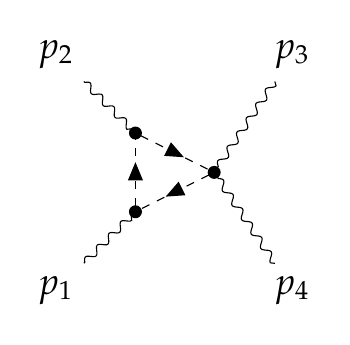
\begin{tikzpicture}[baseline=(current bounding box.center)]
  \begin{feynman}
    \vertex[dot] (v1) at (-0.5,-0.5) {};
    \vertex[dot] (v2) at (-0.5,0.5) {};
    \vertex[dot] (v3) at (0.5,0) {};
    \vertex (i1) at (-1.5, -1.5) {$p_1$};
    \vertex (i2) at (-1.5, 1.5) {$p_2$};
    \vertex (f1) at (1.5, 1.5) {$p_3$};
    \vertex (f2) at (1.5, -1.5) {$p_4$};
    \draw[photon] (i1) -- (v1);
    \draw[photon] (i2) -- (v2);
    \draw[photon] (v3) -- (f1);
    \draw[photon] (v3) -- (f2);
    \draw[charged scalar] (v1) -- (v2);
    \draw[charged scalar] (v2) -- (v3);
    \draw[charged scalar] (v3) -- (v1);
  \end{feynman}
\end{tikzpicture}
\hspace{1cm}
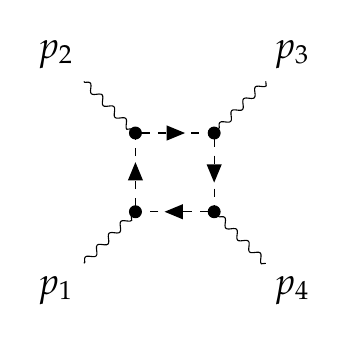
\begin{tikzpicture}[baseline=(current bounding box.center)]
  \begin{feynman}
    \vertex[dot] (v1) at (-0.5,-0.5) {};
    \vertex[dot] (v2) at (-0.5,0.5) {};
    \vertex[dot] (v3) at (0.5,0.5) {};
    \vertex[dot] (v4) at (0.5,-0.5) {};
    \vertex (i1) at (-1.5, -1.5) {$p_1$};
    \vertex (i2) at (-1.5, 1.5) {$p_2$};
    \vertex (f1) at (1.5, 1.5) {$p_3$};
    \vertex (f2) at (1.5, -1.5) {$p_4$};
    \draw[photon] (i1) -- (v1);
    \draw[photon] (i2) -- (v2);
    \draw[photon] (v3) -- (f1);
    \draw[photon] (v4) -- (f2);
    \draw[charged scalar] (v1) -- (v2);
    \draw[charged scalar] (v2) -- (v3);
    \draw[charged scalar] (v3) -- (v4);
    \draw[charged scalar] (v4) -- (v1);
  \end{feynman}
\end{tikzpicture}
\end{center}
Each of these diagrams has a different number of permutations over external momenta. From left to right, we name them $i\mathcal{M}_{1,2,3}(p_i, \epsilon^i)$.
For $i\mathcal{M}_1$ we get the three options of the Mandelstam channels:
\begin{equation}
\begin{gathered}
    i\mathcal{M}_{I} = i\mathcal{M}_1
    + i\mathcal{M}_1(p_2 \leftrightarrow p_4)
    + i\mathcal{M}_1(p_2 \leftrightarrow p_3)
\end{gathered}
\end{equation}
For $i\mathcal{M}_2$ we get all possible permutations of a circle with a start position (just regular order, $4!$), but with two of the photons being at the same place, dividing it by 2 to give 12 options:
\begin{equation}
\begin{gathered}
    i\mathcal{M}_{II} = i\mathcal{M}_2
    + i\mathcal{M}_2(p_2 \leftrightarrow p_3)
    + i\mathcal{M}_2(p_2 \leftrightarrow p_4)
    + \\
    + i\mathcal{M}_2(p_1 \leftrightarrow p_2)
    + i\mathcal{M}_2(p_1 \leftrightarrow p_3)
    + i\mathcal{M}_2(p_1 \leftrightarrow p_4)
    + \\
    + i\mathcal{M}_2(p_2 \leftrightarrow p_4, p_1 \leftrightarrow p_3)
    + i\mathcal{M}_2(p_2 \leftrightarrow p_3, p_1 \leftrightarrow p_4)
    + \\
    + i\mathcal{M}_2(p_1 \rightarrow p_2 \rightarrow p_3 \rightarrow p_1)
    + i\mathcal{M}_2(p_1 \rightarrow p_3 \rightarrow p_2 \rightarrow p_1)
    + \\
    + i\mathcal{M}_2(p_1 \rightarrow p_2 \rightarrow p_4 \rightarrow p_1)
    + i\mathcal{M}_2(p_1 \rightarrow p_4 \rightarrow p_2 \rightarrow p_1)
\end{gathered}
\end{equation}
 For $i\mathcal{M}_3$ we get all permutations of orders in a circle, a total of six:
\begin{equation}
\begin{gathered}
    i\mathcal{M}_{III} = i\mathcal{M}_3
    + i\mathcal{M}_3(p_2 \leftrightarrow p_4)
    + i\mathcal{M}_3(p_2 \leftrightarrow p_4)
    + \\
    + i\mathcal{M}_3(p_3 \leftrightarrow p_4)
    + i\mathcal{M}_3(p_2 \rightarrow p_3 \rightarrow p_4 \rightarrow p_2)
    + i\mathcal{M}_3(p_2 \rightarrow p_4 \rightarrow p_3 \rightarrow p_2)
\end{gathered}
\end{equation}
\subsection{Calculating in the special case $p_i = 0$}
The first diagram gives:
\begin{equation}
    i\mathcal{M}_1 = \epsilon^1_\mu\epsilon^2_\nu (2ie^2)^2\eta_{\mu\nu}\eta_{\sigma\rho} \int \frac{d^dk}{(2\pi)^d} \frac{i}{k^2 - M^2 + i\epsilon}\frac{i}{(k + p_1 + p_2)^2 - M^2 + i\epsilon} \epsilon^{3*}_\sigma\epsilon^{4*}_\rho
\end{equation}
But, using $p_1 = p_2 = 0$, this becomes:
\begin{equation}
    i\mathcal{M}_1 = \epsilon^1_\mu\epsilon^2_\nu (2ie^2)^2\eta_{\mu\nu}\eta_{\sigma\rho} \int \frac{d^dk}{(2\pi)^d} \left(\frac{i}{k^2 - M^2 + i\epsilon}\right)^2 \epsilon^{3*}_\sigma\epsilon^{4*}_\rho
\end{equation}
Moving to Eucliden coordinates and performing the integral using the formula given:
\begin{equation}
    i\mathcal{M}_1 = i4e^4 \frac{\Gamma\left(2 - \frac{d}{2}\right)}{(2\pi)^{d/2}\Gamma(2)}(M^2)^{\frac{d}{2} - 2}\epsilon^1_\mu\epsilon^2_\mu\epsilon^{3*}_\nu\epsilon^{4*}_\nu
\end{equation}
There are two additional permutations, their sum can be written as:
\begin{equation}
    i\mathcal{M}_{I} = i4e^4 \frac{\Gamma\left(2 - \frac{d}{2}\right)}{(2\pi)^{d/2}}(M^2)^{\frac{d}{2} - 2} \varepsilon
\end{equation}
Where we defined:
\begin{equation}
    \varepsilon = \left(
        \epsilon^1_\mu\epsilon^2_\mu\epsilon^{3*}_\nu\epsilon^{4*}_\nu +
        \epsilon^1_\mu\epsilon^2_\nu\epsilon^{3*}_\mu\epsilon^{4*}_\nu +
        \epsilon^1_\mu\epsilon^2_\nu\epsilon^{3*}_\nu\epsilon^{4*}_\mu
    \right)
\end{equation}
The second diagram gives (after taking the momenta to be zero again, causing the entire internal loop to have the same momentum):
\begin{equation}
\begin{gathered}
    i\mathcal{M}_2 = \epsilon^1_\mu\epsilon^2_\nu (-ie)^2(2ie^2)\eta_{\sigma\rho} \int \frac{d^dk}{(2\pi)^d} (2k)^\mu(2k)^\nu \left(\frac{i}{k^2 - M^2 + i\epsilon}\right)^3 \epsilon^{3*}_\sigma\epsilon^{4*}_\rho = \\ =
     -8e^4\int \frac{d^dk}{(2\pi)^d} k^\mu k^\nu \left(\frac{1}{k^2 - M^2 + i\epsilon}\right)^3 \epsilon^1_\mu\epsilon^2_\nu \epsilon^{3*}_\sigma\epsilon^{4*}_\sigma = \\ =
    -\frac{8}{d}e^4 \int \frac{d^dk}{(2\pi)^d} \frac{k^2 }{\left(k^2 - M^2 + i\epsilon\right)^3} \epsilon^1_\mu\epsilon^2_\mu \epsilon^{3*}_\nu\epsilon^{4*}_\nu
\end{gathered}
\end{equation}
Where in the last line we used:
\begin{equation}
    \eta_{\mu\nu} \int d^dk k^2 f(k^2) =  C \int d^dk k_\mu k_\mu f(k^2)
\end{equation}
\begin{equation}
    \eta^{\mu\nu} \eta_{\mu\nu} \int d^dk k^2 f(k^2) =  C \eta^{\mu\nu}\int d^dk k_\mu k_\mu f(k^2)
\end{equation}
\begin{equation}
    d \int d^dk k^2 f(k^2) =  C\int d^dk k^2 f(k^2)
\end{equation}
\begin{equation}
    d = C
\end{equation}
\begin{equation}
    \eta_{\mu\nu} \int d^dk k^2 f(k^2) =  d \int d^dk k_\mu k_\mu f(k^2)
\end{equation}
Moving to Euclidean space and solving the integral gives:
\begin{equation}
    i\mathcal{M}_2 = i\frac{8}{d}e^4 \frac{d}{2} \frac{\Gamma\left(3 - \frac{d}{2} - 1\right)}{(2\pi)^{d/2}\Gamma(3)}(M^2)^{\frac{d}{2} + 1 - 3}\epsilon^1_\mu\epsilon^2_\mu\epsilon^{3*}_\nu\epsilon^{4*}_\nu
\end{equation}
\begin{equation}
    i\mathcal{M}_2 = i2e^4 \frac{\Gamma\left(2 - \frac{d}{2}\right)}{(2\pi)^{d/2}}(M^2)^{\frac{d}{2} - 2}\epsilon^1_\mu\epsilon^2_\mu\epsilon^{3*}_\nu\epsilon^{4*}_\nu
\end{equation}
There are twelve combinations this time. Four of them will give off each of the pairings of polarizations, so we get a factor of three:
\begin{equation}
    i\mathcal{M}_{II} = i16e^4 \frac{\Gamma\left(2 - \frac{d}{2}\right)}{(2\pi)^{d/2}}(M^2)^{\frac{d}{2} - 2}\varepsilon
\end{equation}
Finally, we perform the third diagram:
\begin{equation}
\begin{gathered}
    iM_3 = \epsilon^1_\mu\epsilon^2_\nu (-ie)^4 \int \frac{d^dk}{(2\pi)^d} (2k)^\mu(2k)^\nu (2k)^\sigma(2k)^\rho \left(\frac{i}{k^2 - M^2 + i\epsilon}\right)^4 \epsilon^{3*}_\sigma\epsilon^{4*}_\rho = \\ =
     16e^4 \int \frac{d^dk}{(2\pi)^d} k^\mu k^\nu k^\sigma k^\rho \frac{1}{\left(k^2 - M^2 + i\epsilon\right)^4} \epsilon^1_\mu\epsilon^2_\nu\epsilon^{3*}_\sigma\epsilon^{4*}_\rho
\end{gathered}
\end{equation}
Performing the same trick:
\begin{equation}
    C \int \frac{d^dk}{(2\pi)^d} k^\mu k^\nu k^\sigma k^\rho f(k^2) = \left(\eta_{\mu\nu}\eta_{\rho\sigma} + \eta_{\mu\rho}\eta_{\nu\sigma} + \eta_{\mu\sigma}\eta_{\rho\nu}\right)\int \frac{d^dk}{(2\pi)^d} f(k^2)
\end{equation}
Multiplying both sides by $\eta^{\mu\nu}\eta^{\rho\sigma}$, we get:
\begin{equation}
    C \int \frac{d^dk}{(2\pi)^d} (k^2)^2 f(k^2) = \left(d^2 + 2d\right)\int \frac{d^dk}{(2\pi)^d} f(k^2)
\end{equation}
\begin{equation}
    C = d(d + 2)
\end{equation}
This gives:
\begin{equation}
    iM_3 = \frac{16}{d(d + 2)}e^4 \int \frac{d^dk}{(2\pi)^d} \frac{(k^2)^2}{\left(k^2 - M^2 + i\epsilon\right)^4} \varepsilon
\end{equation}
Moving the Euclidean space and performing the integral using the formula:
\begin{equation}
    iM_3 = i\frac{16}{d(d + 2)}e^4 \frac{d(d + 2)}{4} \frac{\Gamma\left(4 - \frac{d}{2} - 2\right)}{(2\pi)^{d/2}\Gamma(4)}(M^2)^{\frac{d}{2} + 2 - 4} \varepsilon
\end{equation}
\begin{equation}
    iM_3 = i4e^4 \frac{\Gamma\left(2 - \frac{d}{2}\right)}{(2\pi)^{d/2}\Gamma(4)}(M^2)^{\frac{d}{2} - 2} \varepsilon
\end{equation}
Adding all six option together cancels the $\Gamma(4) = 6$ in the denominator, giving:
\begin{equation}
    i\mathcal{M}_{III} = i4e^4 \frac{\Gamma\left(2 - \frac{d}{2}\right)}{(2\pi)^{d/2}}(M^2)^{\frac{d}{2} - 2} \varepsilon
\end{equation}
Adding all three of them together gives:
\begin{equation}
    i\mathcal{M} = i24e^4 \frac{\Gamma\left(2 - \frac{d}{2}\right)}{(2\pi)^{d/2}}(M^2)^{\frac{d}{2} - 2} \varepsilon
\end{equation}
\subsection{The effective action at low momenta}
\subsubsection{The contribution of the term from 2.1 (a)}
The term we wrote $-\frac{g}{16}F_{\mu\nu}^4$ contributes directly to the four photon scattering amplitude at tree level. However, since the term has derivatives, the contribution of the vertex is zero for $p_i = 0$ (it has a multiplicative factor $((p^\mu + p^\nu)^2)^2$).
\subsection{The mismatch}
It seems that the result from our calculation is not matched to the generic form of an effective action in low momenta for a photon-only effective theory, since the most general terms we wrote are still related to derivatives and thus cancel out.
\newline
This is a result of taking the momenta to zero, since for photons, this is not a physical limit. 
\subsection{Imaginary part of the $2 \rightarrow 2$ scattering amplitude}
For any non zero momenta, since for these values there exists some $q$ such that $(p_1 + p_2)^2 \ge 4q^2$ so a photon pair with momenta $q$ and $-q$ can be created and annihilated as an intermidiate physical state. 
\newpage
\section{Spontaneous symmetry breaking}
\subsection{Feynman rules for the effetive theory}
These are the Feynman rules for scalar fields theory. So, for every diagram:
\begin{itemize}
    \item Each $\sigma$ propagator gives $\frac{i}{p^2 -2\mu^2 + i\epsilon}$.
    \item Each $\pi_a$ propagator gives $\frac{i}{p^2 + i\epsilon}$, since the $\pi_a$ fields don't have a mass term.
\end{itemize}
There are then five types of vertices ($\sigma$ is a solid line and $\pi_a$ are dashed lines):
\begin{center}
\begin{tikzpicture}[baseline=(current bounding box.center)]
  \begin{feynman}
    \vertex (v1) at (-0.5, 1) {$\sigma$};
    \vertex (v2) at (-0.5, -1) {$\sigma$};
    \vertex (v3) at (1, 0) {$\sigma$};
    \vertex (center) at (0, 0);
    \draw[plain] (v1) -- (center);
    \draw[plain] (v2) -- (center);
    \draw[plain] (v3) -- (center);
  \end{feynman}
\end{tikzpicture}
\hspace{1cm}
\begin{tikzpicture}[baseline=(current bounding box.center)]
  \begin{feynman}
    \vertex (v1) at (-0.5, 1) {$\pi_a$};
    \vertex (v2) at (-0.5, -1) {$\pi_a$};
    \vertex (v3) at (1, 0) {$\sigma$};
    \vertex (center) at (0, 0);
    \draw[dashed] (v1) -- (center);
    \draw[dashed] (v2) -- (center);
    \draw[plain] (v3) -- (center);
  \end{feynman}
\end{tikzpicture}
\hspace{1cm}
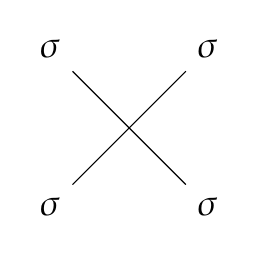
\begin{tikzpicture}[baseline=(current bounding box.center)]
  \begin{feynman}
    \vertex (v1) at (-1, 1) {$\sigma$};
    \vertex (v2) at (-1, -1) {$\sigma$};
    \vertex (v3) at (1, 1) {$\sigma$};
    \vertex (v4) at (1, -1) {$\sigma$};
    \vertex (center) at (0, 0);
    \draw[plain] (v1) -- (center);
    \draw[plain] (v2) -- (center);
    \draw[plain] (v3) -- (center);
    \draw[plain] (v4) -- (center);
  \end{feynman}
\end{tikzpicture}
\hspace{1cm}
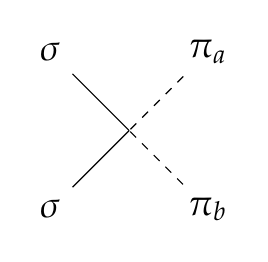
\begin{tikzpicture}[baseline=(current bounding box.center)]
  \begin{feynman}
    \vertex (v1) at (-1, 1) {$\sigma$};
    \vertex (v2) at (-1, -1) {$\sigma$};
    \vertex (v3) at (1, 1) {$\pi_a$};
    \vertex (v4) at (1, -1) {$\pi_b$};
    \vertex (center) at (0, 0);
    \draw[plain] (v1) -- (center);
    \draw[plain] (v2) -- (center);
    \draw[scalar] (v3) -- (center);
    \draw[scalar] (v4) -- (center);
  \end{feynman}
\end{tikzpicture}
\hspace{1cm}
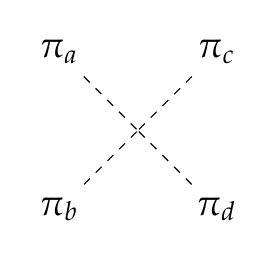
\begin{tikzpicture}[baseline=(current bounding box.center)]
  \begin{feynman}
    \vertex (v1) at (-1, 1) {$\pi_a$};
    \vertex (v2) at (-1, -1) {$\pi_b$};
    \vertex (v3) at (1, 1) {$\pi_c$};
    \vertex (v4) at (1, -1) {$\pi_d$};
    \vertex (center) at (0, 0);
    \draw[scalar] (v1) -- (center);
    \draw[scalar] (v2) -- (center);
    \draw[scalar] (v3) -- (center);
    \draw[scalar] (v4) -- (center);
  \end{feynman}
\end{tikzpicture}
\hspace{1cm}
\end{center}
These give, from left to right. The operators in the Lagrangians don't all have the full combinatorical prefactor, so some get an additional prefactor here:
\begin{itemize}
    \item $\sigma^3 \rightarrow -i6\sqrt{\lambda}\mu$
    \item $\pi_a\pi_b\sigma \rightarrow -i2\sqrt{\lambda}\mu\delta_{ab}$
    \item $\sigma^4 \rightarrow -i6\lambda$
    \item $\pi_a\pi_b\sigma^2 \rightarrow -i2\lambda\delta_{ab}$
    \item $\pi_a\pi_b\pi_c\pi_d \rightarrow -i6\lambda\left(\delta_{ab}\delta_{cd} + \delta_{ac}\delta_{bd} + \delta_{ad}\delta_{bc}\right)$
\end{itemize}
And, of course:
\begin{itemize}
    \item Add a $(2\pi)^d \delta\left(\sum p_i\right)$ for each vertex
    \item Divide by symmetry factor
    \item Integrate over all undertermined momenta
\end{itemize}
\subsection{Scattering of two Nambu-Goldstone bosons}
Using the above vertices, we can see that there is a single vertex that has a tree-level contribution, which is the $\pi_a^4$ vertex, and another vertex that can give contribution at the same order in $\lambda$, but with a loop, which is the $\sigma \pi_a^2$ vertex. This second vertex gives the three Mandelstam channels:
\begin{center}
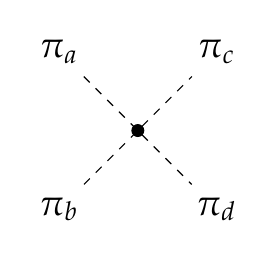
\begin{tikzpicture}[baseline=(current bounding box.center)]
  \begin{feynman}
    \vertex[dot] (v) at (0,0) {};
    \vertex (i1) at (-1, -1) {$\pi_b$};
    \vertex (i2) at (-1, 1) {$\pi_a$};
    \vertex (f1) at (1, 1) {$\pi_c$};
    \vertex (f2) at (1, -1) {$\pi_d$};
    \draw[scalar] (i1) -- (v);
    \draw[scalar] (i2) -- (v);
    \draw[scalar] (v) -- (f1);
    \draw[scalar] (v) -- (f2);
  \end{feynman}
\end{tikzpicture}
\hspace{1cm}
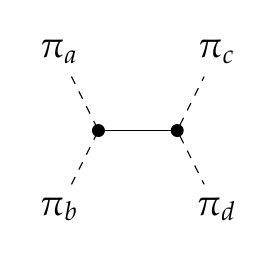
\begin{tikzpicture}[baseline=(current bounding box.center)]
  \begin{feynman}
    \vertex[dot] (v1) at (-0.5,0) {};
    \vertex[dot] (v2) at (0.5,0) {};
    \vertex (i1) at (-1, -1) {$\pi_b$};
    \vertex (i2) at (-1, 1) {$\pi_a$};
    \vertex (f1) at (1, 1) {$\pi_c$};
    \vertex (f2) at (1, -1) {$\pi_d$};
    \draw[scalar] (i2) -- (v1);
    \draw[scalar] (i1) -- (v1);
    \draw[scalar] (v2) -- (f1);
    \draw[scalar] (v2) -- (f2);
    \draw[plain] (v1) -- (v2);
  \end{feynman}
\end{tikzpicture}
\hspace{1cm}
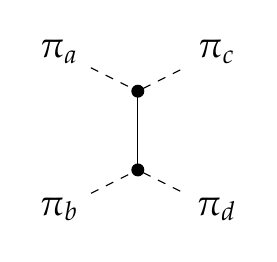
\begin{tikzpicture}[baseline=(current bounding box.center)]
  \begin{feynman}
    \vertex[dot] (v1) at (0,-0.5) {};
    \vertex[dot] (v2) at (0,0.5) {};
    \vertex (i1) at (-1, -1) {$\pi_b$};
    \vertex (i2) at (-1, 1) {$\pi_a$};
    \vertex (f1) at (1, 1) {$\pi_c$};
    \vertex (f2) at (1, -1) {$\pi_d$};
    \draw[scalar] (i2) -- (v2);
    \draw[scalar] (i1) -- (v1);
    \draw[scalar] (v2) -- (f1);
    \draw[scalar] (v1) -- (f2);
    \draw[plain] (v1) -- (v2);
  \end{feynman}
\end{tikzpicture}
\hspace{1cm}
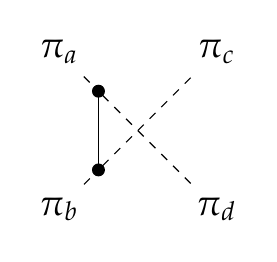
\begin{tikzpicture}[baseline=(current bounding box.center)]
  \begin{feynman}
    \vertex (i1) at (-1, -1) {$\pi_b$};
    \vertex (i2) at (-1, 1) {$\pi_a$};
    \vertex (f1) at (1, 1) {$\pi_c$};
    \vertex (f2) at (1, -1) {$\pi_d$};
    \vertex[dot] (v1) at (-0.5, 0.5) {};
    \vertex[dot] (v2) at (-0.5, -0.5) {};
    \vertex (v0) at (0,0);
    \draw[scalar] (i2) -- (v1);
    \draw[scalar] (i1) -- (v2);
    \draw[scalar] (v0) -- (f1);
    \draw[scalar] (v0) -- (f2);
    \draw[scalar] (v2) -- (v0);
    \draw[scalar] (v1) -- (v0);
    \draw[plain] (v2) -- (v1);
  \end{feynman}
\end{tikzpicture}
\end{center}
This will give:
\begin{equation}
\begin{gathered}
    i\mathcal{M}_{abcd} = -i6\lambda\left(\delta_{ab}\delta_{cd} + \delta_{ac}\delta_{bd} + \delta_{ad}\delta_{bc}\right) - \\ - 4\lambda\mu^2 \left[\delta_{ab}\delta_{cd}\frac{i}{s - 2\mu^2 + i\epsilon} + \delta_{ac}\delta_{bd}\frac{i}{t - 2\mu^2 + i\epsilon} + \delta_{ad}\delta_{bc}\frac{i}{u - 2\mu^2 + i\epsilon}\right]
\end{gathered}
\end{equation}
Now, for $p_i^2 = 0$, we can write $p_i = (\epsilon_i, \vec{p}_i)$, and since $\epsilon_i^2 - \vec{p}_i^2 = 0$ this gives $p_i = (|\vec{p}_i|, \vec{p}_i)$. In the COM system, we can write $\vec{p}_1 = -\vec{p}_2 \equiv \vec{p}_i$ and $\vec{p}_3 = -\vec{p}_4 \equiv \vec{p}_f$. And since $p_1 + p_2 = p_3 + p_4$, we get $\left|\vec{p}_i\right| = \left|\vec{p}_f\right| \equiv p$. Now we can write:
\begin{equation}
    p_1 = (p, \vec{p}_i)
    \qquad
    p_2 = (p, -\vec{p}_i)
    \qquad
    p_3 = (p, \vec{p}_f)
    \qquad
    p_4 = (p, -\vec{p}_f)
\end{equation}
\begin{equation}
    s = 4p^2 \qquad t = u = (\vec{p}_i - \vec{p}_f)^2 = 2p^2 - 2\vec{p}_i\cdot\vec{p}_f = 2p^2 \left(1 - cos\theta\right)
\end{equation}
Where $\theta$ is the collision angle. So, we get:
\begin{equation}
\begin{gathered}
    i\mathcal{M}_{abcd} = -i6\lambda\left(\delta_{ab}\delta_{cd} + \delta_{ac}\delta_{bd} + \delta_{ad}\delta_{bc}\right) - i2\lambda\mu^2 \left[\frac{\delta_{ab}\delta_{cd}}{2p^2 - \mu^2 + i\epsilon} + \frac{\delta_{ac}\delta_{bd} + \delta_{ad}\delta_{bc}}{p^2 \left(1 - cos\theta\right) - \mu^2 + i\epsilon}\right]
\end{gathered}
\end{equation}
\subsection{For zero momentum}
In the $\vec{p}_i = 0$ case, we can write $p = 0$ or $s = t = u = 0$, giving:
\begin{equation}
\begin{gathered}
    i\mathcal{M}_{abcd} = -i6\lambda\left(\delta_{ab}\delta_{cd} + \delta_{ac}\delta_{bd} + \delta_{ad}\delta_{bc}\right) - i2\lambda\mu^2 \left[\frac{\delta_{ab}\delta_{cd}}{- \mu^2 + i\epsilon} + \frac{\delta_{ac}\delta_{bd} + \delta_{ad}\delta_{bc}}{- \mu^2 + i\epsilon}\right] = \\ = -i4\lambda\left[\delta_{ab}\delta_{cd} + \delta_{ac}\delta_{bd} + \delta_{ad}\delta_{bc}\right]
\end{gathered}
\end{equation}
In the case of two fields, for instance $a = b \ne c = d$ (any permutation will yiled the same result), we get:
\begin{equation}
    \mathcal{M} = -4\lambda
\end{equation}
In the case of all fields being the same $a = b = c = d$, we get:
\begin{equation}
    \mathcal{M} = -12\lambda
\end{equation}
\subsection{For small momentum}
For small momenta, using:
\begin{equation}
    \frac{1}{x - \mu^2} \approx -\left(\frac{1}{\mu^2} + \frac{x}{\mu^4}\right)
\end{equation}
We get:
\begin{equation}
\begin{gathered}
    i\mathcal{M}_{abcd} = -i6\lambda\left(\delta_{ab}\delta_{cd} + \delta_{ac}\delta_{bd} + \delta_{ad}\delta_{bc}\right) - \\ + i2\lambda\mu^2 \left[\delta_{ab}\delta_{cd}\left(\frac{1}{\mu^2} + \frac{p^2}{\mu^4}\right) + \left(\delta_{ac}\delta_{bd} + \delta_{ad}\delta_{bc}\right)\left(
        \frac{1}{\mu^2} + \frac{p^2\left(1 - \cos\theta\right)}{\mu^4}
    \right)\right] = \\ =
     -i4\lambda\left(\delta_{ab}\delta_{cd} + \delta_{ac}\delta_{bd} + \delta_{ad}\delta_{bc}\right) + i2\lambda \left[\delta_{ab}\delta_{cd} + \left(\delta_{ac}\delta_{bd} + \delta_{ad}\delta_{bc}\right)\left(1 - \cos\theta\right)
    \right]\frac{p^2}{\mu^2}
\end{gathered}
\end{equation}
For $a = b \ne c = d$:
\begin{equation}
    \mathcal{M} = -4\lambda + 2\lambda \left(\frac{p}{\mu}\right)^2
\end{equation}
For $a = c \ne b = d$ or $a = d \ne b = c$, we get:
\begin{equation}
    \mathcal{M} = -4\lambda + 2\lambda\left(1 - \cos\theta\right)\left(\frac{p}{\mu}\right)^2
\end{equation}
And for $a = b = c = d$, we get both:
\begin{equation}
    \mathcal{M} = -4\lambda + 2\lambda\left(3 - 2\cos\theta\right)\left(\frac{p}{\mu}\right)^2
\end{equation}
The amplitude is not zero, since there is a mixing of the fields, even in small momenta.
\subsection{Symmetry breaking term}
\subsubsection{Global symmetry}
This term breaks the same $SO(N)$ symmetry that was broken when close to the minima, so we get the $SO(N-1)$ rotating all scalar fields except $\Psi_N$, only now it is borken explicitly in the Lagrangian, and not just for small momenta.
\subsubsection{The classical potential minimum}
We can write the classic potential:
\begin{equation}
    V(\Phi^i) = -\frac{1}{2}\mu^2\Phi_i^2 + \frac{\lambda}{4}\left[\Phi_i^2\right]^2 + \alpha \Phi_N
\end{equation}
Taking the derivative with respect to $\Phi_N$ is now different, giving:
\begin{equation}
        \frac{\partial V}{\partial\Phi_N} = -\mu^2\Phi_N + \lambda\Phi_i^2\Phi_N + \alpha
\end{equation}
Taking this to be zero we get the minima for all fields:
\begin{equation}
    \Phi_N\left(\mu^2 - \lambda\Phi_i^2\right) = \alpha
\end{equation}
This is still an $N-1$ dimensional manifold, and therefore this doesn't give an additional symmetry breaking.
\subsubsection{The mass of the fields around the minima in leading order}
% TODO fix this based on the board comment
Let us choose a minimum from the manifold. We will choose:
\begin{equation}
    \Phi_i = \left(0, ..., \frac{\alpha}{\mu^2}\right)
\end{equation}
* The time is over and I finally got here. I know this choice is illegal, since it doesn't solve the above equation. For some reason I forgot that $\Phi_i$ inside the paranthases includes $\Phi_N$ as well when I solved this. I would just solve it in perturbation theory as suggested if I had time, then plug it in. I suppose the mass I would recieve is different, maybe zero, but the calculations are the same.
\newline
We can now take the same expansion around the minimum we would have taken in the regular SSB case:
\begin{equation}
    \Phi_i = (\Pi_k, v + \sigma)
    \qquad
    v = \frac{\alpha}{\mu^2}
\end{equation}
And plug it into the Lagrangian. The mass term will give the fields their original mass:
\begin{equation}
\begin{gathered}
    \frac{1}{2}\mu^2\Phi_i^2 = \frac{1}{2}\mu^2\Pi_i^2 + \frac{1}{2}\mu^2\left(v + \sigma\right)^2 =
    \frac{1}{2}\mu^2\Pi_i^2 + \frac{1}{2}\mu^2\sigma^2 + \mu^2v\sigma + \frac{1}{2}v^2
\end{gathered}
\end{equation}
While the part from the interaction term that has the fields interacting with $v$ reduces their mass:
\begin{equation}
    -\frac{\lambda}{4} \left[\Phi^2\right](v + \sigma)^2 = 
    -\frac{\lambda}{4} \left[\Phi^2\right]v^2 + \cdots = 
    -\frac{\lambda}{4} \left[\Phi^2\right]\frac{\alpha^2}{\mu^4} + \cdots
\end{equation}
S, depending on $\alpha$, the fields might still have mass. Their mass term is:
\begin{equation}
    \frac{1}{2}\left(\mu^2 - \frac{\alpha^2}{2\mu^4}\right)\Phi_i^2
\end{equation}
\end{document}